\documentclass[conference]{IEEEtran}
\IEEEoverridecommandlockouts

\usepackage{cite}
\usepackage{amsmath,amssymb,amsfonts}
\usepackage{algorithmic}
\usepackage{graphicx}
\usepackage{textcomp}
\usepackage{xcolor}
\usepackage{listings}
\usepackage{booktabs}

% ------------------------------------------------------------------
% NOTE ON BIBLIOGRAPHY: this file keeps the \cite keys of the ECML
% submission (e.g. 4815280, qwen3technicalreport). Restore that .bib
% and add the NEW keys listed at the end of this file (prefix-tuning /
% frozen-LM references). The template thebibliography was removed.
% ------------------------------------------------------------------

% ---- Dataset funnel numbers (single source of truth for the text) ----
\newcommand{\FunnelTotal}{67{,}662}        % source items consumed
\newcommand{\NAccepted}{5{,}296}           % validated pairs
\newcommand{\NTrain}{4{,}764}
\newcommand{\NTest}{532}

\def\BibTeX{{\rm B\kern-.05em{\sc i\kern-.025em b}\kern-.08em
    T\kern-.1667em\lower.7ex\hbox{E}\kern-.125emX}}

\begin{document}

\title{Execution-Validated Pseudocode for MATLAB:\\
Dataset Construction and a Diagnosis of\\
Soft-Prefix Collapse in Code Comprehension}

\author{
\IEEEauthorblockN{1\textsuperscript{st} Given Name Surname}
\IEEEauthorblockA{\textit{dept. name of organization (of Aff.)} \\
\textit{name of organization (of Aff.)}\\
City, Country \\
email address or ORCID}
\and
\IEEEauthorblockN{2\textsuperscript{nd} Given Name Surname}
\IEEEauthorblockA{\textit{dept. name of organization (of Aff.)} \\
\textit{name of organization (of Aff.)}\\
City, Country \\
email address or ORCID}
}

\maketitle

\begin{abstract}
Large-scale code-comprehension corpora annotate source code with natural-language descriptions written by a language model, but such annotations are only trusted, not verified: a description can be fluent and still misstate what the program computes. We present a MATLAB$\to$pseudocode dataset in which every annotation carries an \emph{executable proof of faithfulness}. A description is accepted only if a second, independent model---given the description alone---can regenerate code whose output, under execution in Octave on identical inputs, matches the output of the original program. A static resolvability check closes the soundness hole that otherwise corrupts such round-trip validation: functions that call repository-local helpers absent from the corpus are rejected before execution, so no annotation is validated against a fabricated or unexercised dependency. From \FunnelTotal{} corpus functions the pipeline retains \NAccepted{} validated pairs, a stronger acceptance criterion than the $n$-gram similarity or LLM-judge screening used by existing pseudocode corpora. We then use the dataset for a controlled study of a widely assumed design: conditioning a language-model decoder on compressed soft prefixes---a recursive neural network (RvNN) vector over the abstract syntax tree, Vision-Transformer-style patches over CodeBERT embeddings, and their combination---in place of the code's token sequence. The result is strongly negative. A fine-tuned text-only decoder reaches 0.416 ROUGE-L, while all three prefix-conditioned variants collapse to 0.17--0.18, generating a generic template largely independent of the input: they name the function they describe in 0\% of samples (text-only: 80\%), and up to 29\% of their outputs share an identical eight-word opening. We trace the collapse to a capacity asymmetry---2.2B decoder parameters were trainable against a prefix of at most six vectors, making memorization of the unconditional pseudocode distribution cheaper than learning to read the prefix---compounded by prefix bandwidth, an instruction that references absent code, and missing end-of-sequence supervision. The dataset, pipeline, and diagnosis together offer both a verified resource and a cautionary result for structure-injection designs.
\end{abstract}

\begin{IEEEkeywords}
Dataset Construction, Execution-Based Validation, Large Language Model, Code Comprehension, Abstract Syntax Tree, Pseudocode Generation
\end{IEEEkeywords}

% ==================================================================
\section{Introduction}
\label{sec:intro}

Understanding source code is a central activity in software engineering: developers spend much of their effort reading unfamiliar systems, tracing legacy behaviour, debugging, and documenting before they change anything \cite{4815280,10.1147/sj.282.0294,Fjeldstad1979,ko2007information}. Large Language Models (LLMs) have become the dominant tool for automating parts of this work, producing summaries, explanations, and pseudocode from raw source \cite{yuan2023evaluatinginstructiontunedlargelanguage}. Progress on the task, however, is gated by a data problem that is easy to state and hard to solve: \emph{supervised comprehension corpora need natural-language descriptions of code, descriptions at scale are written by LLMs, and LLM-written descriptions are unverified}. A generated description can be grammatical, plausible, and wrong---omitting a branch, inventing a step, or misreading an operator---and a model trained on such targets learns to reproduce plausible unfaithfulness. Existing corpora screen their annotations by $n$-gram similarity to references or by asking another LLM to judge quality; both measure surface agreement, not behaviour.

This paper makes the acceptance criterion behavioural. We construct a MATLAB$\to$pseudocode dataset in which a description is admitted only if it passes a \emph{round-trip execution test}: a second, independent model, given the description and nothing else, must write code whose output under execution matches the output of the original program on identical inputs. Faithfulness of text is thereby reduced to behavioural equivalence of two programs, which can be checked automatically in GNU Octave. Every one of the \NAccepted{} retained pairs carries a concrete artefact of this proof---the original code, the description, the regenerated code, the harness, and both matching outputs.

Round-trip validation has a failure mode that, to our knowledge, prior work does not address, and closing it is a key contribution of the pipeline. Real-world corpora store one function per file, so a function that calls a \emph{repository-local helper}---defined elsewhere in its original project---can never run standalone. When such a function enters a naive round-trip validator, the validation does not fail cleanly; it passes for the wrong reason: either the harness generator silently invents the missing helper, or the chosen inputs never reach the call site, so a ``passing'' execution validates code that does not run as written. We remove these cases \emph{before} any execution or LLM call with a static resolvability check that queries the runtime for every name used in call position. Section~\ref{sec:dataset} quantifies how many candidates this single check removes.

We choose MATLAB as the target language deliberately. It is widely used in control engineering, signal processing, and scientific computing, yet under-represented in LLM pretraining corpora \cite{qwen3technicalreport}, so it is a setting where curated supervision matters most; at the same time the pipeline itself is language-agnostic---it needs only a parser and an interpreter---and MATLAB's interpreter (Octave) is free and scriptable, which makes execution-based acceptance practical at corpus scale.

The second half of the paper uses the dataset for a controlled study of a design assumption common to structure-aware code models: that a compressed continuous representation of a program---an AST summary vector, patch-aggregated encoder embeddings---can stand in for the program's token sequence as conditioning for a language-model decoder. We compare a fine-tuned text-only decoder against three variants that replace the code text with soft prefixes: a single RvNN-encoded AST vector, ViT-style patches over CodeBERT embeddings, and the two combined. The outcome is unambiguous and negative: the text-only decoder reaches 0.416 ROUGE-L while all three prefix variants collapse to 0.16--0.18, and inspection shows they emit a generic template largely independent of the input program. Rather than reporting the numbers and stopping, we diagnose the collapse (Section~\ref{sec:diagnosis}): the deepest cause is a \emph{capacity asymmetry}---2.2B decoder parameters were trainable against a prefix of at most six vectors on 4{,}764 training samples, so memorizing the unconditional distribution of MATLAB pseudocode lowered the loss more cheaply than learning to decode opaque vectors---compounded by the narrow prefix, an instruction that points at code which is not there, and targets that never teach the model to stop.

The contributions of this paper are:
\begin{itemize}
    \item \textbf{An execution-validated MATLAB$\to$pseudocode dataset} of \NAccepted{} pairs, in which every annotation is accepted only when an independent model can reconstruct behaviourally equivalent code from it, together with the full validation artefacts per sample. The dataset and pipeline are public.\footnote{\texttt{https://huggingface.co/datasets/philip120/sc-matlab-validated}}
    \item \textbf{A validation pipeline with a soundness guarantee}: a static resolvability check that prevents non-self-contained functions from producing hollow validations, plus a quantified acceptance funnel showing where candidates are lost.
    \item \textbf{A controlled negative result with a causal diagnosis}: three compressed soft-prefix conditioning schemes all collapse to input-independent template generation on this task, and we identify the training-capacity asymmetry, prefix bandwidth, instruction grounding, and end-of-sequence supervision failures that jointly produce the collapse---each verifiable from our released evaluation outputs.
\end{itemize}

We frame the study around three questions:
\begin{description}
    \item[\textbf{RQ1.}] \textit{Can round-trip execution equivalence validate LLM-generated pseudocode at corpus scale, and what does its acceptance funnel look like?}
    \item[\textbf{RQ2.}] \textit{How well does straightforward decoder fine-tuning perform on execution-validated MATLAB$\to$pseudocode data?}
    \item[\textbf{RQ3.}] \textit{Do compressed structural or patch-based soft prefixes carry enough signal to replace the code's token sequence as decoder conditioning?}
\end{description}

% ==================================================================
\section{Related Work}
\label{sec:related}

\textbf{Code comprehension and summarization.} Code comprehension research spans static analysis, AST-based techniques, statistical models, and, recently, LLMs \cite{husak2025combiningstaticanalysistechniques,SIRBU2025125821,sun2023abstractsyntaxtreeprogramming,4815280}. Evaluation practice ranges from task time and comprehension-question accuracy to automatic overlap metrics \cite{2411.14491,feitelson2021considerations,boehm1978quantitative}. Our task formulation---pseudocode generation as a measurable proxy for comprehension---follows this line, but our focus is on the trustworthiness of the supervision itself.

\textbf{Validation of generated annotations.} Large code--text corpora pair code with docstrings or LLM-generated descriptions, screened (if at all) by heuristic filters, $n$-gram similarity, or LLM-as-judge scoring \cite{yuan2023evaluatinginstructiontunedlargelanguage}. Execution-based signals have been used to validate \emph{generated code} against tests \cite{chen2018execution,shojaee2023execution}; we invert the direction and use execution to validate \emph{generated text}: the description is the artefact under test, and regenerated code is the measurement instrument. To our knowledge, no existing pseudocode corpus admits annotations by behavioural round-trip, nor guards that round-trip against unresolvable dependencies.

\textbf{Structure-aware code models.} A substantial literature injects ASTs into neural code models \cite{10.1007/s10664-023-10378-9,shi-etal-2021-cast,10.5555/3304222.3304348,10.5555/3524938.3524962,10.1109/ICSE43902.2021.00026}, and pre-trained encoders such as CodeBERT and CodeT5 \cite{wang-etal-2021-codet5} supply node- or token-level representations. Patch-style aggregation of embeddings follows the Vision Transformer recipe; its application to code generation is comparatively unexplored \cite{soselia2023learning}. Our study is a controlled stress test of the compressed end of this design space.

\textbf{Soft-prefix conditioning and frozen decoders.} Prefix and prompt tuning condition a language model through learned continuous vectors \cite{li2021prefix,lester2021power}. Multimodal systems that bridge a frozen LLM through a learned projector---Frozen \cite{tsimpoukelli2021frozen}, BLIP-2's Q-Former \cite{li2023blip2}---freeze the decoder precisely so that the training signal is forced through the projected prefix. Our negative result is an empirical demonstration of what happens when that discipline is dropped: with the decoder unfrozen, the model satisfies the objective by memorizing the target distribution and ignoring the prefix entirely. We return to this connection in Section~\ref{sec:diagnosis}.

% ==================================================================
\section{Execution-Validated Dataset Construction}
\label{sec:dataset}

\subsection{The Validation Problem}
Our supervision signal is a step-by-step natural-language description of what each MATLAB function does, generated by an LLM (\texttt{gemini-flash-lite}, temperature 0.2). The generation prompt requires the description to be precise enough that ``someone could reimplement the code from the pseudocode alone and get identical outputs,'' to preserve all computed values, loop bounds, conditions, and output statements, and to avoid MATLAB syntax. This is scalable but not trustworthy on its face. We therefore accept a description into the dataset only if it passes an execution-based faithfulness test, so that data quality is decided by behaviour rather than fluency.

\subsection{Round-Trip Execution Equivalence}
The test is a round trip (Fig.~\ref{fig:pipeline-desc}). Given source code $C$, we generate a description $S$; we then hand $S$ to a second generation call that never sees $C$ and ask it to write code $C'$ in the same language purely from the description. If $S$ faithfully captures the behaviour of $C$, then $C'$ should behave like $C$. We check this by execution: both $C$ and $C'$ run under GNU Octave on identical inputs, and $S$ is accepted only when their outputs agree.

Because a bare function produces no observable output, each function is executed inside a generated test harness: a minimal Octave script that seeds the random state (\texttt{rng(42)}), constructs small numeric inputs, calls the function, and displays every return value. The harness prompt explicitly forbids defining, implementing, or stubbing any helper function---it may only construct inputs and make the call---which is what gives the static check of Section~\ref{sec:resolvability} its teeth. The same harness (with the function name adapted if the regeneration renamed it) runs both $C$ and $C'$, so the two programs are observed under identical inputs. Outputs are normalized before comparison---whitespace canonicalized, floating-point values with five or more decimals rounded to four---so trivial formatting differences do not cause spurious rejections.

\begin{figure}[t]
\centering
\fbox{\parbox{0.96\linewidth}{\small
\textbf{Round-trip acceptance test} \\[2pt]
1.\ $C \xrightarrow{\ \text{LLM}\ } S$ \hfill (describe) \\
2.\ $S \xrightarrow{\ \text{independent LLM, never sees } C\ } C'$ \hfill (reimplement) \\
3.\ run $C$ and $C'$ in Octave under one generated harness \\
4.\ accept $S$ iff $\mathrm{normalize}(\mathrm{out}(C)) = \mathrm{normalize}(\mathrm{out}(C'))$
}}
\caption{The acceptance criterion reduces faithfulness of a natural-language description to behavioural equivalence of two programs.}
\label{fig:pipeline-desc}
\end{figure}

\subsection{The Soundness Hole and the Static Resolvability Check}
\label{sec:resolvability}
Round-trip execution has one failure mode that would quietly corrupt the dataset. The source corpus stores one function per file, so any function that calls a repository-local helper---a routine defined elsewhere in its original project---cannot run standalone. Such a function does not fail the validator cleanly; it can \emph{pass for the wrong reason}. Either the harness generator, asked to produce inputs, silently invents the missing helper, so the function is validated against a fabricated dependency; or the chosen inputs never reach the branch containing the call, so the missing routine is never exercised and the ``passing'' run validates nothing. In both cases execution succeeds while the central claim---that the retained code provably runs as written---is hollow.

We close the hole statically, before any execution or LLM call. From each candidate we extract every identifier used in call position, after blanking string literals (a bare \texttt{'} in MATLAB is ambiguous between transpose and quote, and unstripped string contents otherwise masquerade as calls). We then exclude language keywords, locally defined subfunctions, assigned variables, function parameters and outputs, loop iterators, \texttt{global}/\texttt{persistent} declarations, anonymous-function parameters, and struct-field accesses. Every surviving name is submitted to the runtime itself---Octave's \texttt{exist}---and the candidate is rejected if any name fails to resolve to a builtin, an installed package, or a defined function. Resolution results are cached across candidates, so the check costs a few interpreter calls over the whole corpus. This one check removes 18{,}174 items---26.9\% of the entire corpus, more than three candidates for every pair ultimately accepted---each of which had already passed the quality and dependency filters and would otherwise have entered the round-trip with hollow validation (Table~\ref{tab:funnel}).

\subsection{Acceptance Funnel}
\label{sec:funnel}
The full pipeline, in order: (1)~strip comments; (2)~quality bounds (5--100 lines, $\le$4{,}000 characters, $\ge$50\% unique lines); (3)~reject external I/O, GUI, and toolbox dependencies by pattern (\texttt{fopen}, \texttt{imread}, \texttt{plot}, \texttt{system}, \texttt{eval}, toolbox namespaces, \dots); (4)~the static resolvability check; (5)~reject functions with no returnable or printed output; (6)~content-hash deduplication; (7)~the round-trip execution test of Fig.~\ref{fig:pipeline-desc}. Table~\ref{tab:funnel} reports the funnel over the \FunnelTotal{} source items consumed. Static stages were re-executed deterministically over the same corpus range to obtain exact per-stage counts; the LLM/execution stages are reported as their aggregate, since replaying them would require re-querying the annotation model.

\begin{table}[t]
\centering
\caption{Acceptance funnel over \FunnelTotal{} source-corpus items. Stages apply in order; each row counts items dropped at that stage.}
\label{tab:funnel}
\begin{tabular}{lrr}
\toprule
Stage & Dropped & \% of total \\
\midrule
Empty after comment stripping        & 2       & 0.0 \\
Duplicate of an accepted item (hash) & 2{,}784  & 4.1 \\
Quality bounds                       & 24{,}183 & 35.7 \\
External I/O / GUI / toolbox         & 12{,}971 & 19.2 \\
\textbf{Unresolvable callee (static)}& \textbf{18{,}174} & \textbf{26.9} \\
No observable output                 & 8       & 0.0 \\
Round-trip stage (harness, generation, & & \\
\quad execution, or output mismatch) & 4{,}244  & 6.3 \\
\midrule
\textbf{Accepted}                    & \textbf{\NAccepted} & \textbf{7.8} \\
\bottomrule
\end{tabular}
\end{table}

Two readings of the funnel are worth making explicit. First, the static stages do the heavy lifting: of the 9{,}540 items that reach the round trip, 55.5\% pass it---the expensive LLM-and-execution stage runs only on candidates that can actually run. Second, the round trip is still discriminative, rejecting 4{,}244 candidates whose descriptions failed to reconstruct behaviour; these are precisely the unfaithful annotations that similarity screening would have admitted. Notably, all 735 flat scripts that reached the round trip failed it (typically at original-execution time), so the released dataset consists entirely of functions.

Because execution equivalence is checked on one generated input set, it has limited input coverage: it is a \emph{screen}, not a proof of equivalence on all inputs. Its value is that it removes the large majority of unfaithful annotations automatically and cheaply, leaving a small residue for manual review; a random audit sample of 50 accepted pairs is retained with all artefacts for inspection.

\subsection{Dataset Characterization}
\label{sec:characterization}
The released dataset contains \NAccepted{} validated pairs, all MATLAB functions (no flat script survived the full funnel), drawn from the MNBVC MATLAB corpus.\footnote{\texttt{semran1/yulan-code-MNBVC-matlab} on HuggingFace.} Source functions average 24.7 lines (median 18, range 5--100 by construction); descriptions average 314.6 words (median 272, range 47--1{,}052). Each sample ships with seven artefacts: the cleaned source, the description, the regenerated code, the test harness, both execution outputs, and the source-corpus index. The train/test split is 90/10 (\NTrain{}/\NTest{}) and deterministic by content hash, so samples never migrate between splits across releases and the test split was never seen by any training stage in Section~\ref{sec:models}.

Compared with corpora validated by similarity to human references or by LLM judgement, the acceptance criterion here is strictly harder to satisfy: an annotation must contain enough information to \emph{reconstruct the program's behaviour}, not merely to resemble a reference. The cost is yield---7.8\% of source items survive---and a bias toward self-contained numeric code, which we discuss in Section~\ref{sec:threats}.

% ==================================================================
\section{Case Study: Conditioning a Decoder on Compressed Code Representations}
\label{sec:models}

We now use the dataset to test whether compressed continuous representations of a program can replace its token sequence as decoder conditioning. We frame comprehension as translation $f_{\theta}: C \rightarrow S$ from MATLAB source $C$ to pseudocode $S$, generated autoregressively:
\begin{equation}
  P(s_1, \ldots, s_T) = \prod_{t=1}^{T} P(s_t \mid \mathbf{z},\, s_{<t}),
\end{equation}
where $\mathbf{z}$ is the conditioning representation of $C$. Four variants differ only in $\mathbf{z}$; the decoder is Qwen3-4B-Instruct \cite{qwen3technicalreport} (36 layers, hidden size 2560) in every case.

\subsection{Shared Encoder Machinery}
For the three encoder variants, an ANTLR4-generated MATLAB parser converts the source into an AST, from which we extract semantic nodes---function declarations, conditions, loops, assignments---each recording its nesting depth (Table~\ref{tab:nodes}). Each node's text is encoded by frozen CodeBERT into a 768-dimensional CLS vector; these node vectors are the ``pixels'' every encoder variant consumes. A learned projector bridges CodeBERT's space to the decoder's: $f_{\text{proj}}: \mathbb{R}^{768} \rightarrow \mathbb{R}^{2560}$.

\begin{table}[t]
  \centering
  \caption{Semantic nodes extracted for a small example function.}
  \label{tab:nodes}
  \begin{tabular}{c l l}
    \toprule
    Depth & Type & Text \\
    \midrule
    0 & function\_decl & \texttt{function y = test(x)} \\
    1 & if\_condition  & \texttt{if x > 0} \\
    2 & assignment     & \texttt{x = x + 1} \\
    2 & assignment     & \texttt{y = x * 2} \\
    \bottomrule
  \end{tabular}
\end{table}

\subsection{The Four Variants}
\textbf{Text-only (baseline).} The decoder receives the raw code through its own BPE tokenizer (up to 512 tokens), followed by the instruction prompt; no encoder is involved. This is ordinary sequence-to-sequence fine-tuning.

\textbf{Tree.} A recursive neural network (RvNN) folds the AST bottom-up---children are aggregated into their parent with shared weights, nodes wider than 8 children truncated---until the root yields a single vector $\mathbf{z}_{\text{tree}} \in \mathbb{R}^{2560}$ summarizing the program. The decoder input is $[\mathbf{z}_{\text{tree}}; \text{prompt}]$: \emph{one} soft token in place of the code.

\textbf{ViT.} Following the Vision Transformer recipe, node vectors are grouped into patches of $p{=}4$ consecutive nodes, each flattened patch linearly projected to $\mathbb{R}^{2560}$, giving $\lceil N/p \rceil$ soft tokens ($\approx$5 on average) in place of the code.

\textbf{Combined.} The tree vector is prepended to the patch sequence: $[\mathbf{z}_{\text{tree}}; \mathbf{p}_1, \ldots, \mathbf{p}_M; \text{prompt}]$.

Note what the three encoder variants share: the code's token sequence is \emph{absent}. The decoder sees only projected vectors and a 12-token instruction. Total prefix width is 1 vector (Tree), $\approx$5 (ViT), or $\approx$6 (Combined)---a design that compounds CodeBERT's collapse of each statement to one CLS vector with a further $4\times$ patch grouping. This compression is the hypothesis under test, not an accident: RQ3 asks precisely whether so compact a representation can carry the program.

\subsection{Training}
\label{sec:training}
Training is two-stage. \textbf{Stage 1} fine-tunes the decoder on raw code$\to$pseudocode text pairs (5 epochs, lr $2{\times}10^{-4}$, the last 18 of 36 transformer layers plus final norm and \texttt{lm\_head} unfrozen); it is both the Text-only baseline and the initialization for stage 2. \textbf{Stage 2} trains each encoder variant's projector (lr $3{\times}10^{-4}$, 10 epochs) with the same 18 decoder layers unfrozen at a low learning rate ($1{\times}10^{-5}$); CodeBERT is frozen throughout. The objective in both stages is cross-entropy over target tokens only. All models train on the \NTrain{}-sample train split.

Two facts about this configuration, unremarkable at training time, turn out to matter greatly for the outcome and are flagged here for later reference. First, unfreezing 18 decoder layers plus the head makes \textbf{2{,}205{,}713{,}408 parameters trainable in stage 2}, against a conditioning prefix of at most six vectors. Second, the tokenized targets carry \textbf{no end-of-sequence token}, and are truncated at 512 tokens while references average ${\sim}305$ words. Section~\ref{sec:diagnosis} shows both choices' consequences.

% ==================================================================
\section{Experimental Setup}
\label{sec:setup}

Evaluation uses the held-out \NTest{}-sample test split, unseen by every training stage. Generation is greedy with a 512-token cap. We report ROUGE-1/2/L, BLEU, and chrF, plus efficiency metrics (prefix width, KV-cache size, peak VRAM, latency) measured during the same runs. Owing to interrupted evaluation runs, the variants cover different subsets of the test split (Tree and ViT: all \NTest{}; Combined: 180; Text-only: 100); all cross-variant comparisons in Table~\ref{tab:results} are therefore computed on the 100 items common to all four, and we verified that each variant's full-subset mean differs from its common-100 mean by at most 0.006 ROUGE-L. Significance is assessed with a paired bootstrap (10{,}000 resamples) over the common items.

% ==================================================================
\section{Results}
\label{sec:results}

\begin{table}[t]
\centering
\caption{Quality on the 100 test items common to all variants. All encoder-variant deficits vs.\ Text-only are significant at $p < 10^{-4}$ (paired bootstrap). Full-subset ROUGE-L, where larger evaluation sets exist: Tree 0.173 ($n{=}532$), ViT 0.176 ($n{=}532$), Combined 0.182 ($n{=}180$).}
\label{tab:results}
\begin{tabular}{lccccc}
\toprule
Variant & R-1 & R-2 & R-L & BLEU & chrF \\
\midrule
Text-only & \textbf{0.570} & \textbf{0.307} & \textbf{0.416} & \textbf{0.148} & \textbf{0.459} \\
Combined  & 0.288 & 0.070 & 0.182 & 0.036 & 0.263 \\
ViT       & 0.269 & 0.067 & 0.176 & 0.033 & 0.252 \\
Tree      & 0.263 & 0.064 & 0.173 & 0.033 & 0.248 \\
\bottomrule
\end{tabular}
\end{table}

\textbf{RQ2: text fine-tuning works.} The Text-only decoder reaches 0.416 ROUGE-L / 0.570 ROUGE-1 (Table~\ref{tab:results}, Fig.~\ref{fig:quality}). MATLAB's English-based naming and the precision of the validated targets let a straightforwardly fine-tuned decoder produce largely faithful step-by-step descriptions.

\textbf{RQ3: every compressed-prefix variant collapses.} All three encoder variants land in a narrow band at 0.17--0.18 ROUGE-L---less than half the baseline---and the ordering among them (Combined $>$ ViT $>$ Tree) spans only ${\sim}0.009$ ROUGE-L with overlapping confidence intervals, so we draw no conclusion about their relative merits; in particular we do \emph{not} claim that fusing the two encoders helps. The interesting question is why all three fail identically, which Section~\ref{sec:diagnosis} answers: they are not weak describers of the input but describers of \emph{no input at all}.

\textbf{Efficiency.} The prefix compression works exactly as designed---13--18 input vectors versus 242 text tokens (Fig.~\ref{fig:efficiency})---and KV-cache footprints are correspondingly smaller (46 vs.\ 66\,MB). The numbers are reported for completeness, but we attach no value claim to them: compression that discards the signal is not efficiency \cite{soselia2023learning}. Peak VRAM (7.7--8.7\,GB) is dominated by the decoder in all variants; generation speed is ${\sim}19$ tokens/s throughout, and every encoder variant generated up to the 512-token cap on 100\% of samples (Text-only: 96\%)---a symptom analysed below.

\begin{figure}[t]
      \centering
      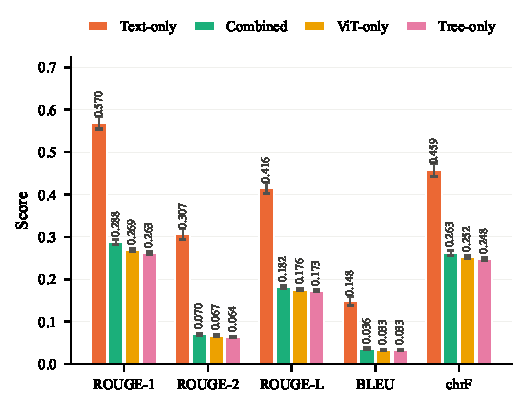
\includegraphics[width=1.0\linewidth]{figures/plot_quality_bars.pdf}
      \caption{Generation quality by variant (test split; bars carry SEM). The text-conditioned baseline more than doubles every metric relative to the three soft-prefix variants.}
      \label{fig:quality}
\end{figure}
\begin{figure}[t]
      \centering
      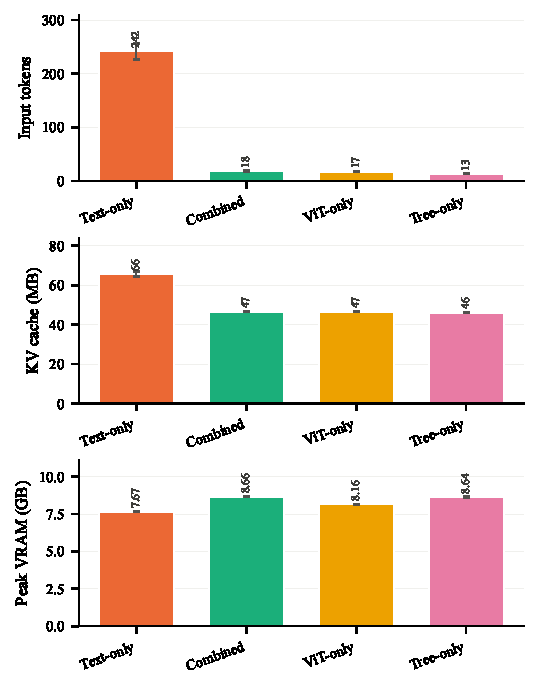
\includegraphics[width=1.0\linewidth]{figures/plot_efficiency.pdf}
      \caption{Efficiency by variant: mean decoder input width, KV-cache size, peak VRAM. The prefix variants achieve the intended ${\sim}13\times$ input compression---while losing the input.}
      \label{fig:efficiency}
\end{figure}

% ==================================================================
\section{Diagnosis: Anatomy of a Prefix Collapse}
\label{sec:diagnosis}

Low overlap scores alone would be compatible with several stories---noisy but input-specific descriptions, systematic verbosity, style mismatch. The stored generations rule those out and identify template collapse.

\subsection{The Generations Are Input-Independent}
Three measurements, each computable from the released evaluation outputs:
\begin{itemize}
    \item \textbf{Function naming.} The Text-only model names the function it is describing in 80\% of common-item samples. All three encoder variants name it in \textbf{0\%}. They do produce function names---confidently, and wrongly: generic hallucinations such as \texttt{get\_size}, \texttt{getdata}, \texttt{sqr}.
    \item \textbf{Shared openings.} 29\% of Tree generations begin with the \emph{identical} eight words (``1.\ Define a function named \texttt{get\_size} that takes''); ViT and Combined show the same degeneracy at 19\% and 9\%. The Text-only model's most common opening appears once.
    \item \textbf{Reference mismatch costs them almost nothing.} Re-scoring encoder-variant generations against randomly mismatched references barely lowers their scores: most of the 0.17 they earn is what any fluent, MATLAB-flavoured, numbered step list earns against this reference distribution.
\end{itemize}

Table~\ref{tab:qualitative} shows the failure concretely: for a rotation-matrix constructor, Text-only describes the actual program, while the three prefix variants fluently describe three different programs that do not exist.

\begin{lstlisting}[language=Matlab]
function R = rotx(t, deg)
if nargin > 1 && strcmp(deg, 'deg')
    t = t*pi/180;
end
ct = cos(t); st = sin(t);
R = [1 0 0; 0 ct -st; 0 st ct];
\end{lstlisting}

\definecolor{refpurple}{HTML}{F0EEFE}
\definecolor{textblue}{HTML}{E8F2FC}
\definecolor{treegreen}{HTML}{E8F8F2}
\definecolor{combinedamber}{HTML}{FEF4E4}
\definecolor{vitred}{HTML}{FDF0F0}
\newcommand{\outbox}[2]{\colorbox{#1}{\parbox{0.95\linewidth}{\small #2}}}

\begin{table}[t]
    \centering
    \caption{Model outputs for the \texttt{rotx} function above (openings shown). The three prefix variants describe hallucinated programs.}
    \label{tab:qualitative}
    \begin{tabular}{p{1.3cm} c p{0.62\linewidth}}
        \toprule
        Variant & R-L & Output (beginning) \\
        \midrule
        Reference & --- &
            \outbox{refpurple}{1.\ Define a function named \texttt{rotx} that takes two inputs: an angle \texttt{t} and an optional parameter \texttt{deg}. 2.\ Check if the number of input arguments is greater than 1 AND if the value of \texttt{deg} equals the string \texttt{'deg'}\ldots} \\[3pt]
        Text-only & 0.60 &
            \outbox{textblue}{1.\ Define a function named \texttt{rotx} that takes two inputs: an angle \texttt{t} and an optional string/flag \texttt{deg}. 2.\ Check if the number of input arguments is greater than 1 AND the value of \texttt{deg} is equal to the string \texttt{'deg'}\ldots} \\[3pt]
        Tree & 0.15 &
            \outbox{treegreen}{1.\ Define a function named \texttt{m2mat} that takes a single input parameter \texttt{x} and returns a value \texttt{y}. 2.\ Check if the number of input arguments provided to the function is less than 2\ldots} \\[3pt]
        ViT & 0.19 &
            \outbox{vitred}{1.\ Define a function named \texttt{getAxes} that takes one input argument, \texttt{nargin}. 2.\ Check if the number of input arguments is less than 2\ldots} \\[3pt]
        Combined & 0.14 &
            \outbox{combinedamber}{1.\ Define a function named \texttt{sqr} that takes a single input argument \texttt{x} and returns a value \texttt{y}. 2.\ Check if the number of input arguments provided is less than 1\ldots} \\
        \bottomrule
    \end{tabular}
\end{table}

\subsection{Four Causes}
\label{sec:causes}
\textbf{C0 --- Capacity asymmetry: the decoder was not frozen.} Stage-2 training unfroze the last 18 decoder layers plus final norm and head: 2{,}205{,}713{,}408 trainable parameters, against a conditioning prefix of at most six vectors, on \NTrain{} samples. Under cross-entropy, two strategies lower the loss: learn to decode six opaque projected vectors, or use two billion parameters to memorize the unconditional distribution of MATLAB pseudocode---every sequence starts ``1.\ Define a function named\ldots'', argument checks follow, loops after that. The second is far cheaper, and it is what training found; the measured degeneracies above are exactly its signature. Systems that successfully condition frozen LLMs through learned projectors---Frozen \cite{tsimpoukelli2021frozen}, BLIP-2 \cite{li2023blip2}, prefix tuning \cite{li2021prefix}---keep the decoder frozen precisely to deny the model this shortcut. This is the deepest cause; the remaining three compound it.

\textbf{C1 --- The prefix is too narrow to compete.} One to six vectors carry the entire program, after CodeBERT has already collapsed each statement to a single CLS vector and patching has grouped statements four at a time. Even a decoder trying to use the prefix has ${\sim}5$ tokens of signal against 12 tokens of fixed prompt. For the prefix to beat memorization it would have to be informative enough to lower per-token loss more than 2.2B parameters of distribution-fitting; at this bandwidth it cannot be.

\textbf{C2 --- The instruction points at nothing.} The decoder input reads $[\text{soft tokens}][\text{``Convert the following MATLAB code\ldots''}][\text{target}]$: the model is told to convert code that \emph{follows}, and nothing follows. The instruction, kept verbatim from the text variant, references an object absent from the sequence, further rewarding the unconditional prior.

\textbf{C3 --- No end-of-sequence supervision.} Targets are tokenized without an EOS token and truncated at 512 tokens against ${\sim}305$-word references, so the model is never trained to stop: 100\% of encoder-variant generations (96\% of Text-only) ran to the decode cap. Fig.~\ref{fig:length-curve} quantifies the cost: score as a function of kept length peaks at 160--240 words for every variant---\emph{before} the cap each hit---against mean generation lengths of 282--328 words. Every model overshoots its own optimum, so raising the cap would lower scores, not raise them; the missing stop token costs accuracy, not budget. This bug affects all four variants equally and therefore cannot explain the baseline--encoder gap; we report it because it caps the baseline's ceiling and because it is cheap to fix.

\begin{figure}[t]
      \centering
      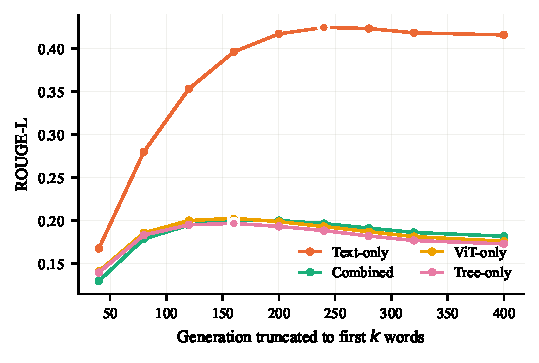
\includegraphics[width=1.0\linewidth]{figures/plot_length_curve.pdf}
      \caption{ROUGE-L as a function of how much of each generation is kept. No end-of-sequence token is appended to training targets, so decoding runs to the token cap on 100\% of encoder-variant samples (96\% for Text-only) and every model overshoots its own optimum: the enlarged marker is each model's peak, reached at 160--240 words against mean generation lengths of 282--328 words.}
      \label{fig:length-curve}
\end{figure}

\subsection{What Would and Would Not Fix It}
The diagnosis implies an ordering of remedies. Fixing C3 (append EOS) is necessary for every variant but would not move the encoders off template behaviour, since it leaves C0--C2 untouched. Fixing C2 (an instruction that references the prefix) is free but similarly insufficient alone. The load-bearing changes are C0 and C1 together: freeze the decoder (or adapt it only through low-rank updates) so the training signal is forced through the projector, and widen the prefix---per-statement rather than per-patch tokens, or structure \emph{alongside} the code text rather than in place of it. A cheap confirmatory probe requiring no retraining is a prefix swap: computing training loss with the correct prefix versus one from a different sample; a near-zero difference would confirm from inside the model that conditioning is dead. We flag this as the first experiment for any follow-up.

% ==================================================================
\section{Discussion}
\label{sec:discussion}

\textbf{For dataset builders.} Round-trip execution equivalence is a practical, automatic acceptance criterion for LLM-generated code annotations: it requires only an interpreter, and it strictly strengthens the guarantee over similarity screening---an accepted description demonstrably contains enough information to reconstruct the program's behaviour. The two lessons that generalize beyond MATLAB: (i) the validator itself must be validated---without the static resolvability check, the 18{,}174 non-self-contained items it removed would have nearly tripled the round-trip pool with candidates whose ``passing'' executions could only be hollow; (ii) yield is the price---at 7.8\%, execution validation is a filter one runs at corpus scale, not a patch one applies to a fixed benchmark.

\textbf{For model builders.} The negative result is a controlled demonstration of a failure mode that is easy to create and expensive to detect: a prefix-conditioned model whose aggregate metrics look like ``weak but working'' (0.17 ROUGE-L is far above zero) while its conditioning is entirely dead. Aggregate overlap metrics did not reveal this; input-dependence probes did---function-naming rate, shared-opening rate, mismatched-reference scoring---and all three are computable from stored generations in minutes, with no baseline construction a reviewer must accept on faith. We suggest them as standard sanity checks for any soft-prefix design.

\textbf{What the dataset enables next.} Because every pair carries its harness and outputs, the dataset supports execution-grounded \emph{model} evaluation---scoring generated pseudocode by whether code regenerated from it reproduces the original outputs---which sidesteps reference-overlap metrics entirely and directly answers the objection that ROUGE against LLM-written references measures style agreement between two language models. Our released pipeline includes this evaluator; applying it to strong text-conditioned models is the natural next study.

% ==================================================================
\section{Threats to Validity}
\label{sec:threats}

\textbf{Annotation source.} Descriptions are written by a single LLM; execution validation bounds their unfaithfulness but not their stylistic homogeneity, and overlap metrics against them partially measure style matching. The execution-grounded evaluation above is the mitigation.

\textbf{Input coverage.} Each pair is validated on one generated input set with a fixed seed; equivalence on those inputs does not imply equivalence everywhere. The criterion is a high-precision screen, not a semantic proof.

\textbf{Selection bias.} The funnel selects self-contained, deterministic, numerically observable functions of 5--100 lines; the dataset under-represents I/O-heavy, toolbox-dependent, and long-form MATLAB, and contains no flat scripts.

\textbf{Single training run.} Each variant was trained once (no multi-seed replication) under one hyperparameter configuration, and the encoder variants share the stage-1 initialization. The diagnosis of Section~\ref{sec:diagnosis} is correspondingly a diagnosis of this configuration---though C0's mechanism (unfrozen decoder out-competing a narrow prefix) is a general hazard, and the checkpoint-restoration path of the evaluator was explicitly verified to load all trained encoder parameters, ruling out an evaluation artefact.

\textbf{Metric ceiling.} The missing-EOS bug (C3) depresses all reported absolute scores; relative comparisons are unaffected since it applies to every variant.

% ==================================================================
\section{Conclusion}

This paper contributes an execution-validated MATLAB$\to$pseudocode dataset---\NAccepted{} pairs in which every annotation is accepted only when an independent model can reconstruct behaviourally equivalent code from it, guarded by a static resolvability check that keeps the validation sound---and a controlled negative result obtained on it: three compressed soft-prefix schemes for injecting code structure into an LLM decoder all collapse to input-independent template generation, while ordinary text fine-tuning performs well. The collapse is not mysterious; it follows from training two billion decoder parameters against a six-vector prefix, and its signature is measurable with three cheap input-dependence probes we recommend to anyone building prefix-conditioned models. The dataset stands independently of the negative result---indeed, because of it: verified supervision is exactly what makes a failure of this kind attributable to the model rather than to the data.

\section*{Acknowledgment}
% TODO: acknowledgments / funding.

% ==================================================================
% BIBLIOGRAPHY
% Restore the .bib from the ECML submission for the existing keys, and ADD
% entries for the new keys cited in Sections II and VII:
%   li2021prefix       - X. L. Li and P. Liang, "Prefix-Tuning: Optimizing
%                        Continuous Prompts for Generation," ACL 2021.
%   lester2021power    - B. Lester, R. Al-Rfou, N. Constant, "The Power of
%                        Scale for Parameter-Efficient Prompt Tuning," EMNLP 2021.
%   tsimpoukelli2021frozen - M. Tsimpoukelli et al., "Multimodal Few-Shot
%                        Learning with Frozen Language Models," NeurIPS 2021.
%   li2023blip2        - J. Li, D. Li, S. Savarese, S. Hoi, "BLIP-2:
%                        Bootstrapping Language-Image Pre-training with Frozen
%                        Image Encoders and Large Language Models," ICML 2023.
% \bibliographystyle{IEEEtran}
% \bibliography{refs}

\end{document}
